\documentclass[tikz, border=10pt]{standalone}

\usetikzlibrary{arrows}

\begin{document}
	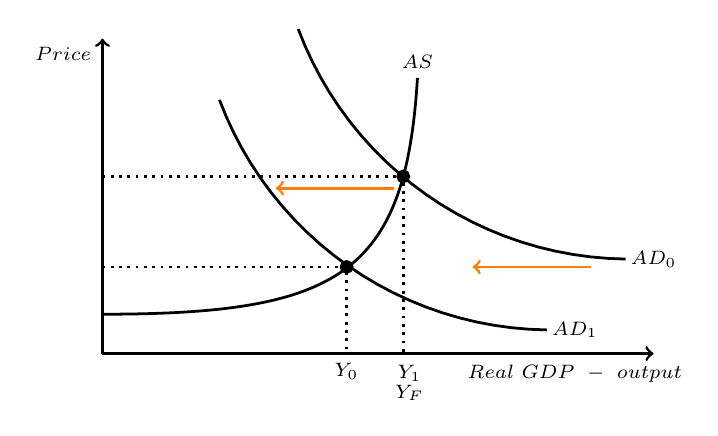
\begin{tikzpicture}[line width=1pt]
	
		\draw[->] (0, 0) -- (7, 0); % Горизонтальная линия
		\draw[->] (0, 0) -- (0, 4); % Вертикальная линия
	
		\draw (0, 0.5) .. controls (3, 0.5) and (3.85, 1) .. (4, 3.5); % Кривая AS
		
		\draw[fill=black] (3.1, 1.1) circle (2pt); 
		\draw[fill=black] (3.82, 2.25) circle (2pt);
		
		\draw [shift={(6.7, 5.7)}] plot[domain=3.5:4.7,variable=\t]({1*4.5*cos(\t r)+-0*4*sin(\t r)},{0*4*cos(\t r)+1*4.5*sin(\t r)});
		\draw [shift={(5.7, 4.8)}] plot[domain=3.5:4.7,variable=\t]({1*4.5*cos(\t r)+-0*4*sin(\t r)},{0*4*cos(\t r)+1*4.5*sin(\t r)});
		
		\draw[dotted] (0, 1.1) -- (3.1, 1.1) -- (3.1, 0);          % Линии P1-Y1
		\draw[dotted] (0, 2.25) -- (3.82, 2.25) -- (3.82, 0); % Линии P2-Y2
		
		
		\draw[<-, color=orange] (2.2, 2.1) -- (3.7, 2.1);
		\draw[<-, color=orange] (4.7, 1.1) -- (6.2, 1.1);

	\begin{scriptsize}
		\draw (-0.5, 3.8) node {$Price$};
		\draw (6, -0.25) node {$Real~GDP~-~output$};
		
		\draw (3.1, -0.225) node {$Y_{0}$};
		
		\draw (3.9, -0.25) node {$Y_{1}$};
		\draw (3.9, -0.5) node {$Y_{F}$};
		
		\draw (4, 3.7) node {$AS$};
		\draw (7, 1.2) node {$AD_{0}$};
		\draw (6, 0.3) node {$AD_{1}$};
	\end{scriptsize}
	\end{tikzpicture}
\end{document}